\documentclass[11pt]{article}
\usepackage{color}
\usepackage{nth}
\usepackage{enumitem}
\usepackage{booktabs}
\usepackage{tabularx}
\usepackage{hyperref}
\usepackage[pdftex]{graphicx}
\usepackage{adjustbox}
\pagestyle{empty}
\setcounter{secnumdepth}{2}
\usepackage{float}

\topmargin=0cm
\oddsidemargin=0cm
\textheight=22.0cm
\textwidth=17cm
\parindent=0cm
\parskip=0.15cm
\topskip=0truecm
\raggedbottom
\abovedisplayskip=3mm
\belowdisplayskip=3mm
\abovedisplayshortskip=0mm
\belowdisplayshortskip=2mm
\normalbaselineskip=12pt
\normalbaselines

% use case stuff
\newcounter{use case ID}

% environment slightly edited from https://tex.stackexchange.com/questions/10293/latex-template-for-use-cases
\newcommand\tabularhead[1]{
    \begin{table}[ht]
        \addtocounter{use case ID}{1}
        \caption{Use Case \arabic{use case ID} - #1}
        \vspace{0.2cm}
        \begin{tabular}{|p{0.2\linewidth}|p{0.70\linewidth}|}
            \hline
            \textbf{Action} & \textbf{#1} \\
            \hline}

        \newcommand\addrow[2]{#1 & #2\\ \hline}

            \newcommand\addmulrow[2]{ \begin{minipage}[t][][t]{2.5cm}#1\end{minipage}
                &\begin{minipage}[t][][t]{11cm}
                    \begin{enumerate}[itemsep=-1ex] #2   \end{enumerate}
                \end{minipage}\vfill\\ \hline}

            \newenvironment{usecase}{\tabularhead}
        {\hline\end{tabular}\end{table}}



        % cheaty non-functional requirement env

        \newcounter{req ID}
        \newcommand\tabularheadfsd[1]{
            \begin{table}[ht]
                \addtocounter{req ID}{1}
                \caption{Non-Functional Requirement \arabic{req ID} - #1}
                \vspace{0.2cm}
                \begin{tabular}{|p{0.2\linewidth}|p{0.70\linewidth}|}
                    \hline
                    \textbf{Action} & \textbf{#1} \\
                    \hline}

                \newenvironment{requirement}{\tabularheadfsd}
                {\hline\end{tabular}\end{table}}

                \begin{document}

                \vspace*{0.5in}
                \centerline{\bf\Large COMP 354}
                \centerline{\bf\Large Requirements for the project 354TheStars}

                \vspace*{0.5in}
                \centerline{\bf\Large Group 5}

                \vspace*{0.5in}
                \centerline{\today}

                \begin{table}[htbp]
                    \caption{Group}
                    \begin{center}
                        \begin{tabular}{|r | c| c |}
                            \hline
                            Name & ID Number & Email \\
                            \hline
                            Morteza Ahmadi & 40038235 & morinob93@gmail.com \\
                            \hline
                            Mohd Tanvir & 40014010 & mohatanvir@hotmail.com \\
                            \hline
                            Arunraj Adlee & 40059206 & arunraj.adlee@hotmail.com \\
                            \hline
                            Dina Sadirmekova & 26321755 & dina.sadirmekova@gmail.com \\
                            \hline
                            Saima Syed & 40044790 & saima.syedb@gmail.com \\
                            \hline
                            Mehdi Skouri Saidi & 40057700 & mehdi879@hotmail.com \\
                            \hline
                            Trevor Lall & 40044047 & trevorlall95@gmail.com \\
                            \hline
                            Stefan John Bosco & 40057206 & johnboscostefan@gmail.com \\
                            \hline
                            Timothy Rodriguez & 40075447 & timmy\_258@hotmail.com \\
                            \hline
                            Lyonel Zamora & 27385986 & yonelz516@gmail.com \\
                            \hline
                            Radhep Sabapathipillai & 40033092 & Radhep.Saba@gmail.com \\
                            \hline
                            Miguel Jimenez & 40022302 & migueleduardo298@hotmail.com\\
                            \hline
                        \end{tabular}
                    \end{center}
                \end{table}

                \begin{table}[htbp]
                    \caption{Revision history}
                    \begin{center}
                        \begin{tabular}{|r | c| c |}
                            \hline
                            Version & Date & Changes \\
                            \hline
                            1.0 & \nth{29} September 2018 & completed requirements \\
                            \hline
                        \end{tabular}
                    \end{center}
                \end{table}


                \tableofcontents
\listoffigures
\clearpage
\listoftables

\clearpage


\section{Document Purpose}

The purpose of this document is to define requirements for the web application 354TheStars. This document may thus be used to orient the development of the application. It seeks to understand the requirements of the problem, formulate the necessary functions and properties needed to answer this problem and its requirements, and then test these functions against the requirements. Hence, it may be used by our users to specify the problem and its requirements, by the developers to understand what functions their system must implement, and what to test their system against. The primary audience for this document are the stakeholders of the project and the development team of the system, as well the project testers for fine-tuning their testing strategy.

\section{Project description}

\subsection{System Context}

Our system will mainly involve the user interacting with a web application interface. The user shall create an account to be able to buy or sell products, however user does not require to have an account for browsing the website. The user information will be stored in a remote database server. Users will not be able to create an account or login by using any social media platforms. It will discussed in more details in future version of this documentation.

\clearpage

\begin{figure}[htbp]
    % \includegraphics[width=\linewidth]{context.png}
    \caption{System Context}
    \label{fig:system-context}
\end{figure}

\subsection{Project Scope}
354TheStars is planning to provide a worldwide platform, where various size of companies as well as individuals can sell or buy products. All of the available products shall be eligible for sale.

\subsection{Business Goals}

\begin{itemize}
    \item \textbf{Compete with existing solutions}

        We are not the sole developers of e-commerce applications by far. As such, if we want to attract users to our platform, we must be able to compete on the same playing field as these current platforms. It is because of that reason, we must, at the very least, provide a secure, easy to use, and performant platform.

    \item \textbf{Reduce service fee}
        We are aiming to empower businesses, and in order to do so, it is necessary to provide a great service and a competitive service fee.

\end{itemize}

\subsection{Product Functions}
\begin{table}[H]
        \caption{Traceability Matrix}
        \begin{adjustbox}{width=\columnwidth,center}
            \begin{tabular}{|r | c| c | c| c|}
                \hline
                ReqID & Category & Requirement & Use Case & User Story \\
                \hline
                R01 & \ Account & A registered user should be able to edit account information & & US02, US03 \\
                    \hline
                R02 & \ Account & A registered should be able to have up to 3 shipping addresses &  & US02, US03 \\ 
                    \hline
                R03 & \ Account & A registered user should be able to view order history &  & US02, US03 \\ 
                \hline
                R04 & \ Account & A registered user should be able to recover user information & &  \\
                \hline
                R05 & \ Account & A new user should be able to sign up & & US02, US03  \\
                \hline
                R06 & \ Account & A new user should receive account creation confirmation email & &  \\
                \hline
                R07 & \ Admin & The administrator should be able to manage user accounts & & US01  \\
                \hline
                R08 & \ Admin & The administrator should be able to manage seller listings &  & US01 \\ 
                \hline
                R09 & \ Buying & A user should be able to add product to shopping cart & UC03 &  \\
                \hline
                R10 & \ Buying & A user should be able to modify shopping cart & UC03 &  \\
                \hline
                R11 & \ Buying & The website should calculate tax & UC03 &  \\
                \hline
                R12 & \ Buying & The buyer should be able to choose shipping method & UC03 &  \\
                \hline
                R13 & \ Buying & A user should be able to pay for product with PayPal & UC2, UC03 & US02, US03 \\
                \hline
                R14 & \ Buying & The website should send purchase confirmation emails with receipt & & US02 \\ 
                \hline
                R15 & \ Buying & A buyer should be able to review a product & UC04 & US02, US03 \\ 
                \hline
                R16 & \ Listing & A user should be able to view product description & & US02, US03, US04 \\ 
                \hline
                R17 & \ Listing & A user should be able to view product photo & & US02, US03, US04 \\ 
                \hline
                R18 & \ Listing & A user should be able to view product rating and review (if any) & & US02, US03, US04 \\
                \hline
                R19 & \ Listing & A user should be able to view product stock count & & US02, US03, US04 \\ 
                \hline
                R20 & \ Listing & A user should be able to view product price & & US02, US03, US04 \\ 
                    \hline
                R21 & \ Interface & The website should contain a search bar & & US02, US04 \\
                \hline
                R22 & \ Interface & A user should be able to sort search results by price  & & US02, US03, US04 \\ 
                \hline
                R23 & \ Interface & A user should be able to sort search results by location  & & US02, US03, US04 \\ 
                \hline
                R24 & \ Interface & A user should be able to sort search results by rating  & & US02, US03, US04 \\ 
                \hline
                R25 & \ Interface & The website should provide a quality UI for the administrator & & US01 \\ 
                \hline
                R26 & \ Interface & A registered user should be able to log in using email or username and password & & US02, US03 \\
                    \hline
                R27 & \ Interface & A user should be able to contact customer support & UC01, UC02, UC03 &  \\
                \hline
                R28 & \ Interface & The website should contain contact information & &  \\
                \hline
                R29 & \ Interface & The website should contain a logo & &  \\
                \hline
                R30 & \ Interface & Homepage should display promotions & &  \\
                \hline
                R31 & \ Interface & Homepage should display products with the most positive reviews & &  \\
                \hline
                R32 & \ Interface & Homepage should highlight the sellers who sell the most & &  \\
                \hline
                R33 & \ Restriction & The system should limit item description characters & UC01 &  \\
                \hline
                R34 & \ Restriction & The website should contain only legal products & &  \\
                \hline
                R35 & \ Restriction & The website should contain only quality descriptions and photos & UC01 &  \\
                \hline
                R36 & \ Restriction & Seller contact information should be hidden & UC03 &  \\
                \hline
                R37 & \ Restriction & Enforce 15 days since purchase period before posting review & UC04 &  \\
                \hline
                R38 & \ Restriction & Enforce the 5 photo per review rule & UC04 &  \\
                \hline
                R39 & \ Restriction & Enforce the 400 character limit for review & UC04 &  \\
                \hline
                R40 & \ Restriction & Ensure that all the required information is correctly filled out & UC01, UC03, UC04 &  \\
                \hline
                R41 & \ Restriction & The homepage shouldn't look too cluttered and busy & &  \\
                \hline
                R42 & \ Restriction & Homepage should not display more than 20 items before pagination begins & &  \\
                \hline
                R43 & \ Restriction & The system should allow only registered user to make a purchase & &  \\
                \hline
                R44 & \ Search & A user should be able to search by name & & US02, US04 \\ 
                \hline
                R45 & \ Search & A user should be able to search by category & & US02, US04 \\ 
                \hline
                R46 & \ Selling & A seller should be able to add products to sell & UC01 & US03 \\
                \hline
                R47 & \ Selling & A seller should be able to edit products information & UC01 & US03 \\ 
                \hline
                R48 & \ Selling & A seller should be able to delete products & UC01 &  \\ 
                \hline
                R49 & \ Selling & The system should allow Bob TheRich to collect 8\% of the sale price & UC02 &  \\
                \hline
                R50 & \ Selling & The seller should be able to allow and disallow returns & UC02 &  \\
                \hline
                R51 & \ Selling & The seller should be able to set time limit for returns & UC02 &  \\
                \hline
                R52 & \ Selling & The seller should receive sale notification & UC02 &  \\
                \hline
                R53 & \ Selling & The seller should be able to mark item as shipped & UC02 &  \\
                \hline
        \end{tabular}
    \end{adjustbox}
\end{table}
\clearpage


\subsection{Personas} \label{actors}
\subsubsection{Admin}
The website administrator maintains the site and has access to manage all the
products and users on 354TheStars. As a representative of the site, their duties include
work with the programming that operates the platform, as well as making sure
everything is running smoothly and according to the rules and code of conduct.
This is the only role not operated or embodied by customers.
\subsubsection{Buyer}
Buyers represent one role of 354TheStars' registered users. Whether they are
an individual or a business, they can search, filter and purchase items from sellers,
which will be delivered to their preferred address. Moreover, they can also review
the products they have acquired from the site and even provide pictures to depict
their feelings and the state of the product received. Finally, buyers will be providing
354TheStars with revenue through a commision acquired from each purchase.
\subsubsection{Guest User}
Guest users are individuals or businesses that are casually visiting 354TheStars,
or future buyers or sellers that have not yet registered themselves on the site.
They have the same privileges as registered users (buyers and sellers) but making
purchases or sales; therefore, for a guest user to complete an order or
to start listing products, they must create an account.
\subsubsection{Seller}
Sellers represent the other possible role of our registered users. Whether they are
an individual or a business, they can list products and provide a description,
images, price and modify their available stock for sale. Lastly, sellers can also
reply to reviews from buyers to better address their customers.
\subsubsection{PayPal}
PayPal is the only actor that is not embodied by a human. PayPal Holdings Inc. is
an American company that operates a worldwide online payment platform. 354TheStars
will be using PayPal's services to process money transactions needed for the purchase
and sale of items on the site. They have no say in the activities or the
decision-making process to mantain and manage 354TheStars, meaning the only
relationship with the site will be of processing payments. Finally, this takes
place by redirecting buyers to PayPal's website for them to input their payment
and billing information to be processed.



\subsection{Functional Requirements} \label{func req}

This section will cover the functional requirements associated with the 354TheStars web application. These are the software capabilities that must be present in order for the user to carry out the services provided by the app or to execute the use cases.

\begin{itemize}
    \item \textbf{Sell:} The system allows a registered user to add product and its details (price, description, image) to be able to sell the product.
    \item \textbf{Buy:} The system allows a registered user to buy a product. Also the buyer can review the purchased product after fifteen days.
    \item  \textbf{Search:} The system allows both a registered user and guest user to browse and search through all the products.
    \item  \textbf{Admin panel:} The admin panel allows the admin to manage, view, and edit user accounts and their information such as (username, email, address, phone number). The panel also allows the admin to manage, view and edit all the products in the website.
    \item \textbf{Purchase process:} The system provides a secure and safe online payment system for buyers. They can use their Paypal account to buy products from the website.
\end{itemize}

\clearpage

% type: quality, quality goals, quality of service, constraint
\subsection{Non-Functional Requirements}\label{nonfunc req}

\begin{requirement}{Interface}
    \addrow{Requirement ID:}{01}
    \addrow{Type:}{Quality of Service}
    \addrow{Description:}{The website should be intuitive, easy to navigate and provide the administrator with a quality experience when accessing and viewing the account information of a user.}
    \addrow{Reasoning:}{If the website is not user-friendly and intuitive to use, the user will feel overwhelmed and have the desire to exit. It should be easy for the administrator to navigate the website, otherwise it would be a challenge to keep the organization up.}
    \addrow{Quality attribute scenario:}{Users should be able to familiarize themselves with the website within seconds of visiting it.}
\end{requirement}

\begin{requirement}{Security}
    \addrow{Requirement ID:}{02}
    \addrow{Type:}{Quality of Service}
    \addrow{Description:}{The application should provide the user with the utmost security. All transactions should be made if and only if valid credentials were provided, if not the service should be denied.}
    \addrow{Reasoning:}{A user should be able to navigate through the application without being concerned about an intruder obtaining access to the user's personal information. The trust built through the level of security provided to the users is what will lead to the success of the application. The user is trusting our service by providing sensitive information such as personal email address, payment information etc. and mishandling this data would greatly damage the business's reputation.  }
    \addrow{Quality attribute scenario:}{All sensitive information should be hidden. The database storing all the personal information needs to be encrypted.}
\end{requirement}

\begin{requirement}{Performance}
    \addrow{Requirement ID:}{03}
    \addrow{Type:}{Quality of Service}
    \addrow{Description:}{The website should run in a smooth fashion. Searching for an item should be quick and efficient.}
    \addrow{Reasoning:}{If the user experiences any problem with searching or posting an item they will not be satisfied.}
    \addrow{Quality attribute scenario:}{No matter how full the database gets the performance should always remain optimal. This will provide a quality experience for the user.}
\end{requirement}

\begin{requirement}{Reliability}
    \addrow{Requirement ID:}{04}
    \addrow{Type:}{Quality of Service}
    \addrow{Description:}{The service should be reliable and functional to the users at all time. If updates need to be made, users will be informed and given enough time to finish any transactions that need to be completed. }
    \addrow{Reasoning:}{Reliability is what will provide users access to the application at all time. If the application is riddled with issues and bugs, users will consider moving to one of the competitors. The business will not and cannot be successful if the users are not provided a fully functional service at all time. }
    \addrow{Quality attribute scenario:}{The system will be online at all times providing services all around the clock. Back up of the system data will provide a continuous run time of the application even if parts of the application were to fail.}
\end{requirement}

\begin{requirement}{Maintainability}
    \addrow{Requirement ID:}{05}
    \addrow{Type:}{Development Constraint}
    \addrow{Description:}{The application should be able to adapt to newer features and innovations that may occur. To maintain the current application, the testing should be divided into multiple instances, before releasing it to production.}
    \addrow{Reasoning:}{Due to the growth in technology, the application should be able to adapt to future changes. The application should also be easy to maintain and make changes to. If a complete tear up is required to apply updates, it becomes an issue. To make it cost effective and future proof, maintainability needs to be easily applied.}
    \addrow{Quality attribute scenario:}{Any changes to the application need to go through the developer server and test server before making out to production. In this manner, we make multiple verifications and avoid downtime due to new updates.}
\end{requirement}

\begin{requirement}{Distribution}
    \addrow{Requirement ID:}{06}
    \addrow{Type:}{Architectural Constraint}
    \addrow{Description:}{The website should work well in both desktop and mobile browsers.}
    \addrow{Reasoning:}{Mobile phones are extremely common. The user should not have a problem navigating it through their phone.}
    \addrow{Quality attribute scenario:}{We are taking advantage of the portability of mobile phones, making sure users can experience the website wherever they have their mobile devices.}
\end{requirement}

\clearpage

\section{User-Stories}

\textbf{User-Story 1 (Admin)} \\
As an admin:
\begin{itemize}
   \item I should be able to create, manage and delete user accounts.
    \item I should have the options to view personal information of the users including:
        \begin{itemize}
            \item Username
            \item Email
            \item Address
            \item Phone Number
        \end{itemize}
    \item I should be able to view and manage every single product that is posted in the website.
    \item The application should provide quality user experience when accessing and viewing account information of a user.
\end{itemize}

\textbf{User-Story 2 (Buyer)} \\
As a buyer:
\begin{itemize}
    \item I should be able to sign up using:
        \begin{itemize}
            \item Username
            \item Email
            \item Address
            \item Phone Number
            \item Password
        \end{itemize}
    \item I should be to edit my personal information.
    \item I should be able to see a product's detail including:
        \begin{itemize}
            \item Image
            \item Description
            \item Price
            \item Reviews
        \end{itemize}
    \item I should have the ability to search for a product by:
        \begin{itemize}
            \item Name
            \item Category
        \end{itemize}
    \item I should be able to filter and sort the search results based on:
        \begin{itemize}
            \item Price
            \item Location
            \item Reviews
        \end{itemize}
    \item I should be able to pay with my PayPal account.
    \item I should get a confirmation email showing a successful purchase.
    \item I should be able to add up to three shipping addresses.
    \item I should be able to add a review to a product after fifteen days of purchasing the product.
    \item I should be able to see my orders history.

\end{itemize}

\textbf{User-Story 3 (Seller)} \\
As a seller:
\begin{itemize}
    \item I should be able to sign up using:
        \begin{itemize}
            \item Email
            \item Username
            \item Address
            \item Phone number
            \item Password
        \end{itemize}
    \item I should be able to edit my personal info including:
        \begin{itemize}
            \item Email
            \item Address
            \item Phone number
            \item Password
        \end{itemize}
    \item I should be able to add a product to sell.
    \item I should be able to edit a product's info including:
        \begin{itemize}
            \item Price
            \item Image
            \item Description
            \item Stock's count
        \end{itemize}
    \item I should have the same ability as a buyer.
\end{itemize}

\clearpage

\textbf{User-Story 4 (Guest User)} \\
As a guest user:
\begin{itemize}
    \item I should be able to browse through products.
    \item I should be able to search for a product by using:
    \begin{itemize}
        \item Name
        \item Category
    \end{itemize}
    \item I should be able to filter and sort the search results based on:
        \begin{itemize}
            \item Price
            \item Location
            \item Reviews
        \end{itemize}
    \item I should be able to see a product's detail including:
        \begin{itemize}
            \item Image
            \item Description
            \item Price
            \item Reviews
        \end{itemize}
\end{itemize}


\section{Glossary of Domain Concepts} \label{glossary}
\begin{table}[H]
    \caption{Glossary of Domain Concepts}
    \begin{center}
        \scalebox{0.7}{
            \begin{tabular}{|l|p{0.8\linewidth}|}
                \hline
                Expression &  Definition \\
                \hline
                Admin & The person who manages the website as well as users and products.  \\
                \hline
                User Account & A data object containing user information including username, email, address(es), phone number. \\
                \hline
                Registered User & The person who has successfully made a user account. \\
                \hline
                Guest User & The person who is not a registered user, however has the ability to browse the website. \\
                \hline
                Product & A legal object that is posted by a seller.\\
                \hline
                Seller & The person who is a registered user and is able to add legal products to sell on the website.\\
                \hline
                Buyer & The person who is a registered user and is able to purchase products on the website.\\
                \hline
                Purchase & A type of transaction where the buyer use to buy a product on the website.\\
                \hline
                Shipping Address & An address that the product will be shipped to after a buyer has successfully purchased a product.\\
                \hline
                PayPal & PayPal Holdings Inc. is an American company that operates a worldwide online payment platform. \\
                \hline
                Database & A local or online container which holds data in an organised, efficient manner. \\
                \hline
                Server & A computer that is accessible on a network, on which a database and/or system may be hosted. The bank institutions' databases will be hosted on here. \\
                \hline

            \end{tabular}}
    \end{center}
\end{table}

\clearpage


\section{Use Cases}
\subsection{Selling}

The use case diagram below represents the Selling functionality of the Online Shopping Website. A detailed description of each use case follows. 

\begin{figure}[htbp]
    \centering
    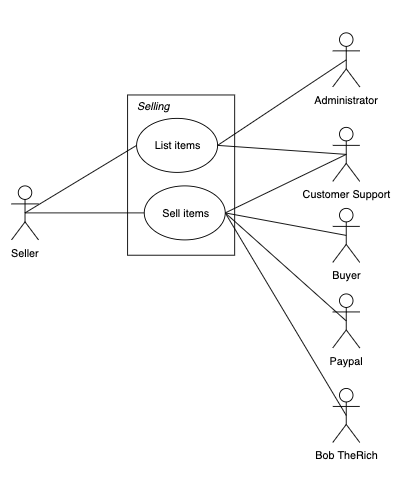
\includegraphics[width=0.5\textwidth]{ucd1.png}
    \caption{Use Case Diagram 1: Online Shopping Website - Selling }
    \label{fig:ucd1}
\end{figure}

\begin{usecase}{List items}
    \addrow{Case ID}{UC01}
    \addrow{Actors}{\textbf{Seller, Administrator, Customer Support}}
    \addrow{Summary}{Seller completes all the information necessary to list an item and has the option to edit or delete it. The Administrator can manage all the listings information. In case of any issues, the Customer Support can be contacted.}
    \addrow{Pre-Conditions}{The user is registered as a legitimate seller.}
    \addrow{Data}{Product photo, product description, price, stock count.}
    \addrow{Stimulus}{Seller pressed on Add Listing/Edit Listing/Delete Listing Button}
    \addmulrow{Response}{
            \item Add Listing/Edit Listing/Delete Listing dialogue appears.
            \item Seller fills out all the information.
            \item Listing added/edited/deleted successfully.
    }
    \addmulrow{Exceptions}{
            \item The required information is not filled out.
            \item The description is over the character limit (100 characters). 
    }
    \addrow{Priority}{High}
    \addmulrow{Open Issues}{
            \item Should the Seller be able to preview the listing?
            \item What happens if the item is illegal? 
            \item How do we check the quality of the image?
            \item How do we check if the seller is legitimate?
    }
\end{usecase}

\begin{usecase}{Sell items}
    \addrow{Case ID}{UC02}
    \addrow{Actors}{\textbf{Seller, Buyer, Paypal, Bob TheRich, Customer Support}}
    \addrow{Summary}{Seller accepts payment for the item from Buyer and pays Bob TheRich the 8\% of the sale fee. The Seller can allow or disallow returns and set the time limit for returns. The Seller and Bob TheRich can access the sales history. In case of any issues, the Customer Support can be contacted.}
    \addrow{Pre-Conditions}{Seller, Buyer, and Bob TheRich must have a valid Paypal account. }
    \addrow{Data}{Paypal account information, sales data, returns option, time limit for returns, 8\% fee, shipped items}
    \addrow{Stimulus}{Buyer paid for item(s)}
    \addmulrow{Response}{
            \item Paypal transfers money from the Buyer account to the Seller Account and sends a confirmation.
            \item Seller receives a sale notification by email.
            \item The sale appears in the Seller’s sales history.
            \item Bob TheRich invoices the Seller for 8\% of the sale. 
            \item Seller pays Bob TheRich through Paypal. 
            \item Seller marks item as shipped. 
    }
        
    \addmulrow{Exceptions}{
            \item Confirmation from Paypal not received.
    }
    \addrow{Priority}{High}
    \addmulrow{Open Issues}{
            \item Should refunds be allowed? If yes, how should they be handled?
            \item What happens if the sale appears in the sales history but not in the shipped items history after a predetermined amount of time?
    }
\end{usecase}
\clearpage

\subsection{Buying}

The use case diagram below represents the Buying functionality of the Online Shopping Website. A detailed description of each use case follows. 

\begin{figure}[htbp]
    \centering
    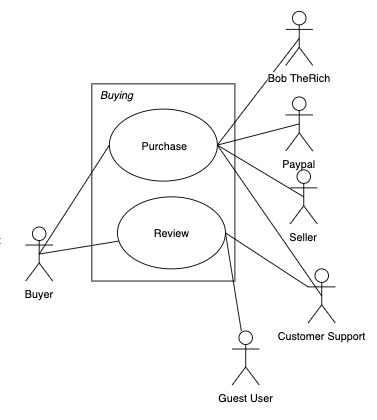
\includegraphics[width=0.5\textwidth]{ucd2.png}
    \caption{Use Case Diagram 1: Online Shopping Website - Buying }
    \label{fig:ucd2}
\end{figure}

\begin{usecase}{Purchase}
    \addrow{Case ID}{UC03}
    \addrow{Actors}{\textbf{Buyer, Seller, Paypal, Bob TheRich, Customer Support}}
    \addrow{Summary}{The Buyer views the shopping cart, has the option to modify it, and pays for it. In case of any issues, the Customer Support can be contacted.}
    \addmulrow{Pre-Conditions}{
        \item Buyer is a registered user.
        \item Buyer has a valid Paypal account. 
        \item Seller contact is hidden.
    }
    \addrow{Data}{Purchase photo, purchase description, purchase quantity, purchase price per item, total purchase price, taxes, shipping fee, shipping address, Paypal account, receipt (Seller information, Buyer information, purchase date, purchase details, purchase price, taxes)}
    \addrow{Stimulus}{Buyer presses the Checkout Button.}
    \addmulrow{Response}{
            \item Buyer views the shopping cart information and can modify it.
            \item Buyer chooses the shipping option (standard or express).
            \item Buyer chooses the shipping address.
            \item Buyer pays the Seller for the purchase through Paypal.
            \item Buyer views the confirmation screen.  
            \item Buyer receives a confirmation and receipt by email.
            \item Order added to the purchase history.
    }
    \addmulrow{Exceptions}{
        \item Any of the required information is missing or incorrect
        \item Buyer exceeded the time limit to complete purchase
        \item Buyer abandons the cart
        \item Buyer did not receive a confirmation screen
    }
    \addrow{Priority}{High}
    \addmulrow{Open Issues}{
        \item What happens if the Buyer is not allowed to purchase the product legally?
    } 
    
\end{usecase}

\begin{usecase}{Review}
    \addrow{Case ID}{UC04}
    \addrow{Actors}{\textbf{Buyer, Guest User, Customer Support}}
    \addrow{Summary}{Buyer leaves a review for a product previously purchased. In case of any issues, the Customer Support can be contacted.}
    \addrow{Pre-Conditions}{
        15 days must have passed since the Buyer’s purchase of the product being reviewed.
        }
    \addrow{Data}{
Review text, review photo, days since purchase, Buyer’s username, rating (out of 5 stars)
}
    \addrow{Stimulus}{Buyer clicks on the Add Review button}
    \addmulrow{Response}{
        \item Buyer rates the product
        \item Buyer adds review text
        \item Buyer adds review photos (optional)
        \item Buyer posts the review
        \item Review appears on the product page for any Guest User to view
    }
    \addmulrow{Exceptions}{
        \item 15 days haven’t passed since the purchase
        \item Buyer posted more than 5 photos per review
        \item Review over the character limit (400 characters)
        \item Any of the required information is missing
    }
    \addrow{Priority}{Medium}
    \addmulrow{Open Issues}{
        \item Should the Buyer be able to preview the review?
        \item How do we handle offensive reviews?
    }
\end{usecase}

\clearpage

\section{Reference}



\begin{itemize}
    \item User information: As our user and use-cases was based on feedback provided by our developers, our references lie mainly within our own team.
    \item Craig Larman - Applying UML and Patterns
    \item Greg Butler's course COMP 354 content
    \item \href{http://web.mit.edu/ssit/cis/CISRequirements.html}{\textcolor{blue}{MIT Curricular Information System
        Software Requirements Document}}
    \item \href{https://resources.sei.cmu.edu/asset_files/TechnicalReport/2005_005_001_14621.pdf}{\textcolor{blue}{Carnegie Mellon Business Goals}}
    \item \href{http://www.oracle.com/technetwork/testcontent/gettingstartedwithusecasemodeling-133857.pdf}{\textcolor{blue}{Use-Case: Oracle }}

\end{itemize}
\end{document}
